\documentclass[12pt,a4paper,oneside]{memoir}
%========================================Packages============================================
\usepackage[ruled,linesnumbered]{algorithm2e}
\usepackage{graphicx}
\usepackage{subcaption}
\usepackage{titlesec}
\usepackage[left=1.25in, right=1in, top=0.75in, bottom=0.75in]{geometry}
\usepackage{setspace}
\usepackage[numbers]{natbib}
\usepackage{pdfpages}
\usepackage{xltabular}
\usepackage{times}
\usepackage{enumitem}
\usepackage{tikz}
\usepackage{listings}
\usepackage{xcolor}
\usepackage{fancyvrb}
\pdfminorversion=7
\DefineVerbatimEnvironment{MyVerbatim}{Verbatim}{breaklines,breakanywhere}

\definecolor{codegreen}{rgb}{0,0.6,0}
\definecolor{codegray}{rgb}{0.5,0.5,0.5}
\definecolor{codepurple}{rgb}{0.58,0,0.82}
\definecolor{backcolour}{rgb}{0.95,0.95,0.92}


\usetikzlibrary{shapes.geometric, arrows, positioning}

\tikzstyle{block} = [rectangle, draw, fill=blue!20, 
    text width=8em, text centered, rounded corners, minimum height=4em]
\tikzstyle{line} = [draw, -latex']
\setSpacing{1.25}
\newcommand\tab[1][0.5cm]{\hspace*{#1}}
%========================================VTU GUIDELINE for chapter section and subsection============================================
\newcommand{\tit}{\fontsize{18}{22}\selectfont}
\newcommand{\chapft}{\fontsize{16}{18}\selectfont}
\newcommand{\secfnt}{\fontsize{16}{18}\selectfont}
\newcommand{\ssecfnt}{\fontsize{14}{16}\selectfont}
\newcommand{\sssecfnt}{\fontsize{12}{14}\selectfont}

\titleformat{\chapter}[display]
  {\normalfont\chapft\bfseries}{\chaptertitlename\ \thechapter}{20pt}{\tit\centering}

\titleformat{\section}
  {\normalfont\secfnt\bfseries}{\thesection}{1em}{\raggedright}

\titleformat{\subsection}
  {\normalfont\ssecfnt\bfseries}{\thesubsection}{1em}{\raggedright}

\titleformat{\subsubsection}
  {\normalfont\sssecfnt\bfseries}{\thesubsubsection}{1em}{\raggedright}

\lstset{
    backgroundcolor=\color{backcolour},   
    commentstyle=\color{codegreen},
    keywordstyle=\color{magenta},
    numberstyle=\tiny\color{codegray},
    stringstyle=\color{codepurple},
    basicstyle=\ttfamily\footnotesize,
    breakatwhitespace=false,         
    breaklines=true,                 
    captionpos=b,                    
    keepspaces=true,                 
    showspaces=false,                
    showstringspaces=false,
    showtabs=false,                  
    tabsize=2,
    language=Python
}

\setsecheadstyle{\secfnt\bfseries\raggedright}
\setsubsecheadstyle{\ssecfnt\bfseries\raggedright}
\setsubsubsecheadstyle{\sssecfnt\bfseries\raggedright}
\setlength{\beforechapskip}{0pt} 
\setlength{\afterchapskip}{20pt} 
\setcounter{tocdepth}{2}
\setcounter{secnumdepth}{3}
\setsecnumdepth{subsection}
%Do not change anything above it
\begin{document}
%======================================Front Pages=========================================================================

\includepdf{PDFs/1_COVER_PAGE.pdf} % Make sure this path is correct

\includepdf{PDFs/2.CERTIFICATE.pdf} % Make sure this path is correct
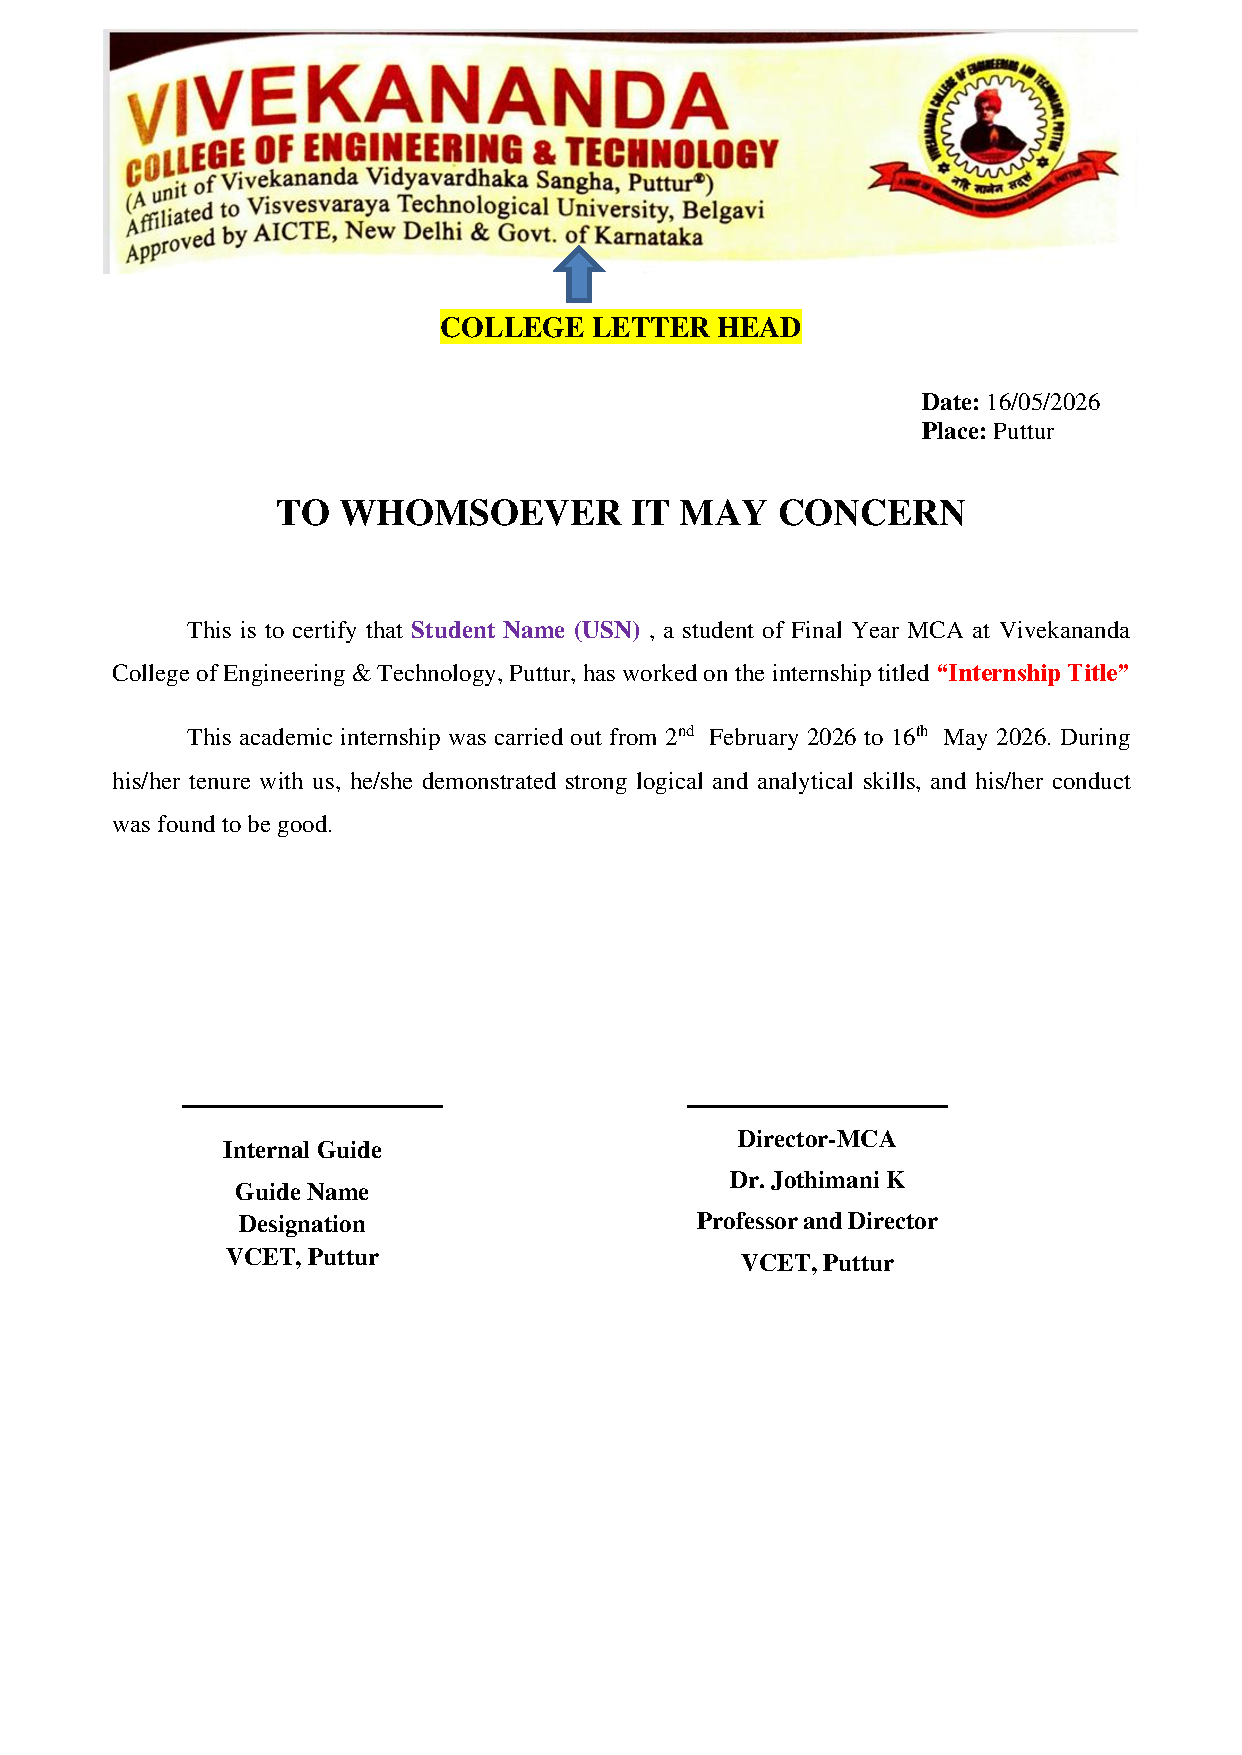
\includepdf{PDFs/3.College Letter.pdf} % Make sure this path is correct

\includepdf{PDFs/4_DECLARATION.pdf} % Make sure this path is correct

\includepdf{PDFs/5_ACKNOWLEDGEMENT.pdf} % Make sure this path is correct
%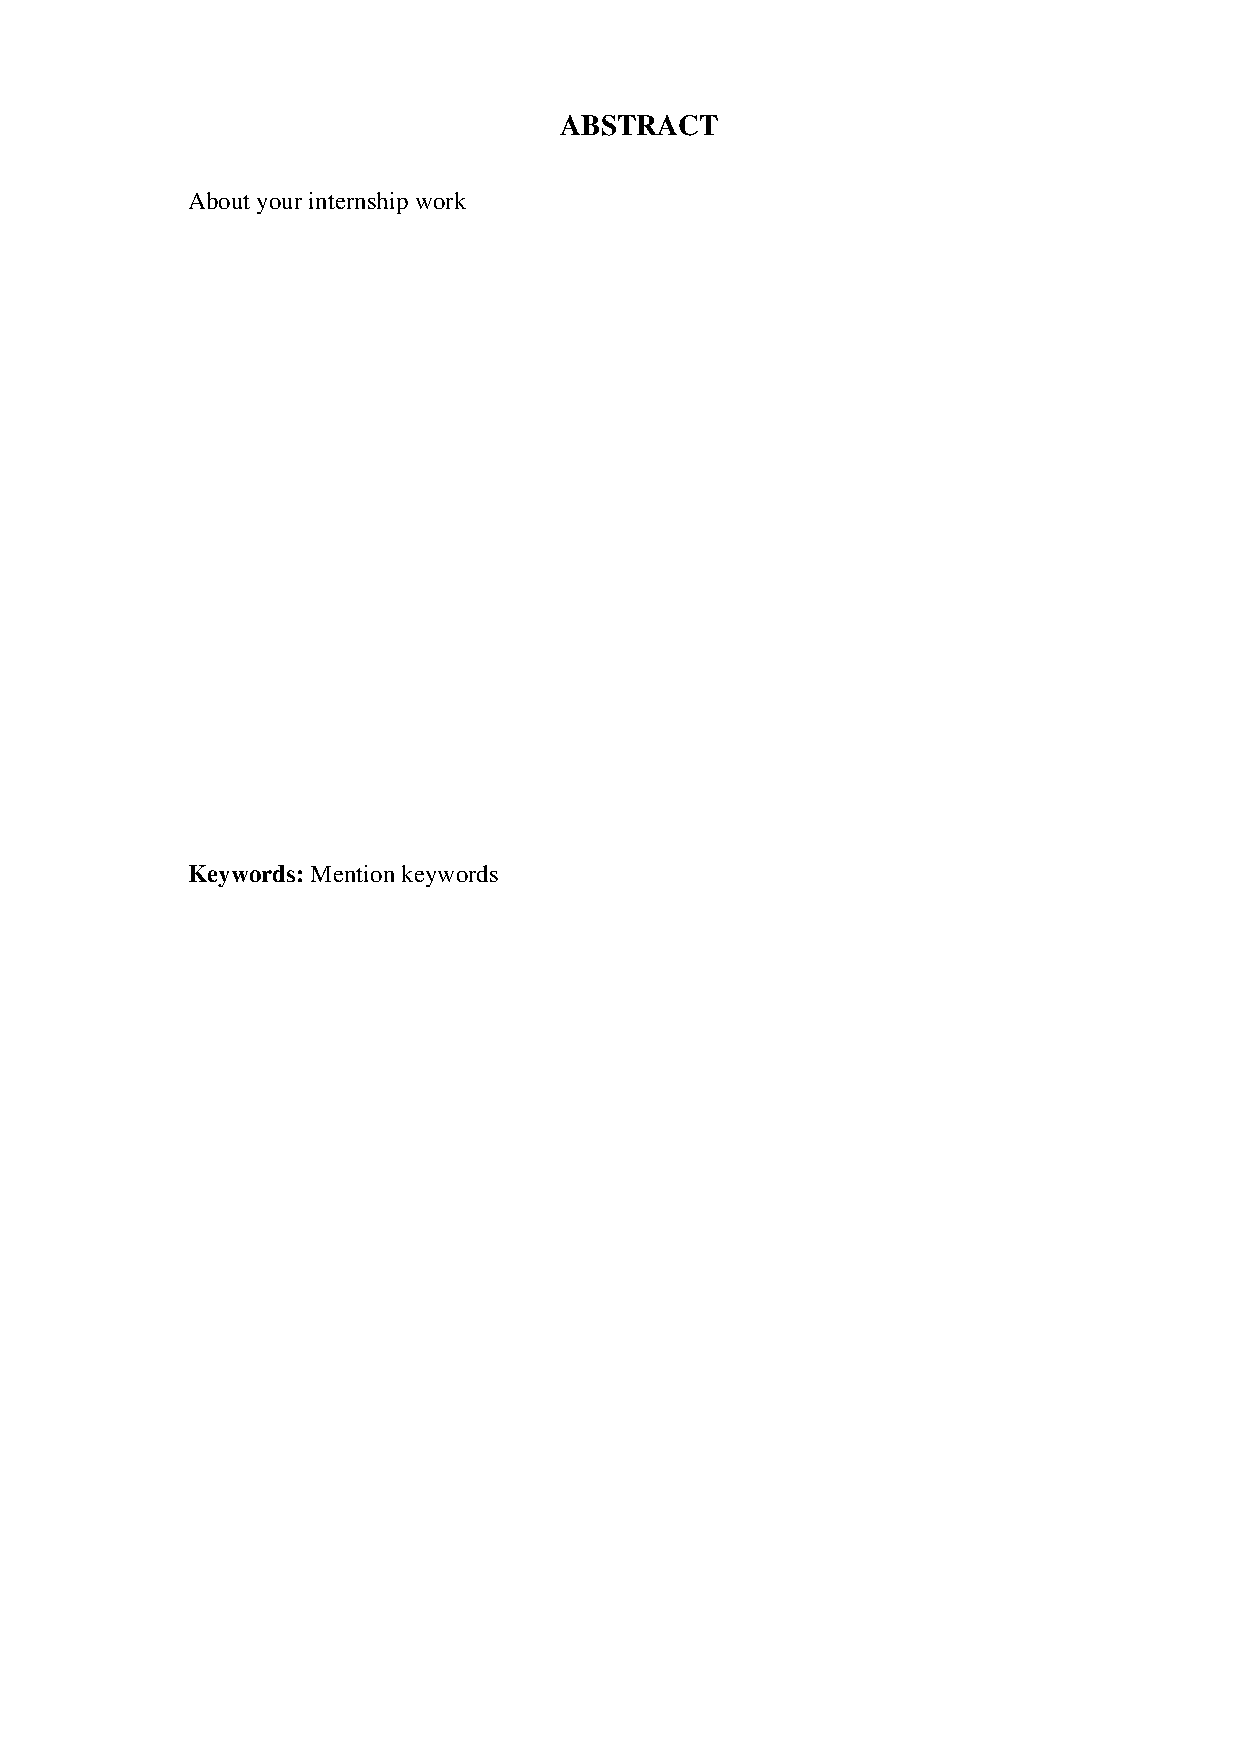
\includepdf{PDFs/6._Abstract.pdf} % Make sure this path is correct

\chapter*{Abstract}

The internship, titled Data Science and AI/ML – MakeX, focuses on applying smart computing technologies to solve real-world problems. With the rapid growth of machine learning and data analysis techniques, sectors such as agriculture, healthcare, and environmental management have seen significant improvements in efficiency and decision-making. The main objective of the internship was to gain hands-on experience in Python programming, data handling, and machine learning concepts. Libraries like NumPy, Pandas, and Matplotlib were used for data preprocessing, analysis, and visualization. As part of the internship, a project titled Plant Leaf Disease Detection System was developed. The system utilizes image processing and deep learning techniques to identify diseases in plant leaves. A Convolutional Neural Network (CNN) model was implemented to classify leaf images as either healthy or diseased. The project included stages such as data collection, preprocessing, model training, evaluation, and deployment. The trained model was then integrated into a user-friendly interface to deliver real-time predictions. Overall, the internship improved technical knowledge, enhanced problem-solving abilities, and provided a better understanding of machine learning applications in agriculture.

\vspace{1em}
\noindent\textbf{Keywords:} Machine Learning, Deep Learning, Computer Vision, CNN, Image Processing, Agriculture

\newpage

\pagestyle{plain}
\pagenumbering{none}
\frontmatter
\pagenumbering{roman}
\renewcommand{\contentsname}{Table of Contents}
\tableofcontents
\newpage
\listoffigures
\newpage
\listoftables 
\newpage
\mainmatter 
\pagenumbering{arabic}
%======================================Header and Footer========================
\pagestyle{myheadings}
\makeheadrule{myheadings}{\textwidth}{0.4pt}
\makefootrule{myheadings}{\textwidth}{0.4pt}{\footruleskip}
\makeoddhead{myheadings}{\small{Internship Title}}{\small{\leftmark}}{\small{2025-26}} % Chnage Title and Academic Year
\makeoddfoot{myheadings}{\small{Department of Master of Computer Applications (MCA), VCET, Puttur}}{}{\small Page {\thepage}}
%======================================Chapter Starts========================
\chapter{Introduction}
\section{Introduction}
Internship topic,Purpose of project,Importance of your work




\section{Company Profile}
Company overview with the following points
\\
\textbf {Name of the Company:}Company Name\\
\textbf{Address:}Address of the company\\
\textbf{Contact Numbers:} contact number\\
\textbf{Email:}mail id\\
\textbf{Services/products:}\\
\textbf{Technologies used:}\\
\textbf{Major projects:}

\begin{comment}
\begin{figure}[h]
    \centering
    \includegraphics[width=0.5\linewidth]{Images/Company Logo.png}
    \caption{\textbf{Company Logo}}
    \label{fig:logo}
\end{figure}

\end{comment}


\chapter{Software Requirements Specification}
\section{Functional Requirements}
    Write what system does:Features of system, for examples:User login, Data processing, Message transmission and so on..

\section{Non Functional Requirements}
    Write system quality aspects:Performance,Security,Scalability, Reliability
\section{Hardware requirements}
\begin{itemize}
\item \textbf{Processor:} Mention
\item \textbf{RAM:}Mention
\item \textbf{Hard Disk:} Mention

....
...
...
and so on
\end{itemize}

\section{Software requirements}
\begin{itemize}
\item \textbf{Operating System:} Mention
\item \textbf{Coding Language:} Mention
\item \textbf{Tool:} Mention
\item \textbf{Editor:} Mention
\item \textbf{Libraries:} Mention

....
...
...
and so on
\end{itemize}
\section{Browser compatibility}
Brief explanation about browser compatibilty
    \begin{itemize}
        \item{\textbf{Supported Browsers: }}Mention
    \end{itemize}
\section{UI Design}Mention UI design languages with explanations in brief(Design approach and Screens layout)
\section{Security Measures}
    \begin{itemize}
        \item{\textbf{Authentication: }}Explain
        \item{\textbf{Data protection: }}Explain
    \end{itemize}
   

\chapter{Project Carried Out}
\section{Project Objectives}
Write  atleast 3 objectives

\section{Methodology}
explain Approach used to complete the project, Development process (which model used to develop..., )
\begin{comment}
\begin{figure}[h]
    \centering
    \includegraphics[width=0.3\linewidth]{Images/overall_diagram.png}
    \caption{\textbf{Block diagram for Overall Methodology}}
    \label{fig:enter-label}
\end{figure}

The figure 3.1 represents  ........explain step by step including data processing and interaction between modules
\begin{figure}[h]
    \centering
    \includegraphics[width=0.3\linewidth]{Images/work_flow.png}
    \caption{\textbf{Workflow diagram for project name}}
    \label{fig:enter-label}
\end{figure}
\end{comment}
The figure 3.2 represents workflow for  ........explain
\section{Modules Developed}
List and explain each module which includes (Module name, Function of module, Input and Output)

\section{Challenges Faced}
explain technical difficulties,debugging issues,learning challenges

\section{Solutions Implemented}
explain how problems were solved and improvements made
\section{Coding}
Add important coding part here..........


\chapter{Results and Conclusion}
\section{Project Assessment and Outcomes}
\begin{comment}
\begin{figure}[h]
    \centering
    \includegraphics[width=0.5\linewidth]{Images/ui_img.png}
    \caption {\textbf{User Interface for ...}}
   \label{fig:ui1}
\end{figure}
\end{comment}
Figure 4.1 dipicts the ........explain 

Also Add screenshots of main pages/modules(atleast 2 to 3 working modules and explain figures in 2 to 3 lines)

\section{Personal Development}
\subsection{Technical Skill Development}
explain New technologies, tools, and concepts learned and Practical implementation knowledge

\subsection{Problem-Solving and Analytical Skills}
explain Ability to identify issues,Debugging and logical thinking improvement

\subsection{Communication Skills}
explain Interaction with mentors and team, Improvement in technical explanation

\subsection{Teamwork and Collaboration}
explain Working in a group, Coordination and cooperation

\subsection{Time Management and Work Discipline}
explain Task planning and execution with below table

\begin{table}[h]
    \centering
    \caption{\textbf{Week-wise Work Progress}}
    \begin{center}  
        %  % \begin{tabular}{|c{}|p{13.0cm}|}
        % \begin{tabular}{|p{1.0cm}|p{13.0cm}|}
        \begin{tabular}{|p{1.5cm}|p{10.0cm}|}
            \hline
            \textbf{Week} & \textbf{Work Progress} \\ \hline
            1 &  ... \\ \hline
            2 & ... \\ \hline
            3 &  ... \\ \hline
            4 &  ... \\ \hline
            5 &  ... \\ \hline
            6 &  ... \\ \hline
            7 & ... \\ \hline
            8 &  ... \\ \hline
            9 &  ... \\ \hline
            10 &  ... \\ \hline
             11 &  ... \\ \hline
            12 & ... \\ \hline
            13 &  ... \\ \hline
       
        \end{tabular}
    \end{center}
    \label{tab:work}
\end{table}
The table 4.1 represents .....summarize...
\newpage
\section{Conclusion}
briefly conclude your work 




\newpage 
%======================================Chapter Ends========================

\renewcommand{\bibname}{References}
\renewcommand{\refname}{References}

\bibliographystyle{unsrtnat}
\begin{thebibliography}{9}
 
 
............Atleast 25 references must include(follow same format refer [1], then cite your work in the report(chapterwise sections))
\end{thebibliography}

\nocite{*}


%========================================================================
\end{document}